\scanpage{55}
% archive sheet number: 54

% L1–5, question
\uline{Question} $X$ espace topologique, $Y$ fermé de $X$, $F$ faisceau \uline{injectif} sur $X$, est-il vrai que $H^i(Y,F|Y)=0$ pour $i>0$ [d'où résulterait que $H^i(V,F|V)=0$ pour tt ouvert $V$ de $Y$, $i>0$]. Réponse \uline{négative}.

% L6–7, after answer
Tout d'abord, il n'est pas vrai que pour un faisceau $F$ sur $X$, \unsure{$=$|même} injectif, l'hom \unsure{(injectif)|(surjectif)}

% L8, restriction
\[
\underset{\substack{U\ \mathrm{vois.}\\ \mathrm{de}\ Y}}{\underrightarrow{\lim}}\ \deleted{\unsure{H}}\ H^0(U,F)\longrightarrow H^0(Y,F)
\]

% L9–11, continuation
soit aussi \uline{surjectif}, i.e. qu'une section se prolonge à un voisinage [i.e. à $X$ tt entier si $F$ est flasque, p.ex. injectif]

% L12–19, first example
\uline{Ex 1} $X$ espace irréductible, $Y$ formé de deux pts fermés distincts \inserted{$a,b$}, $F$ faisceau des applications \unsure{quelc.} dans $\mathbb{Q}$, la section de $F|Y$ qui est le germe $0$ en $a$, le germe $1$ en $b$, ne se prolonge ``pas'' \deleted{\unsure{[à la}} à \deleted{un voisinage} $X$, car si oui la section prolongée serait $0$ sur un voisinage $U$ de $a$, $1$ sur un voisinage $V$ de $b$, or $U\cap V\ne\varnothing$, absurde.

% Left of L14–16, two points
\figure{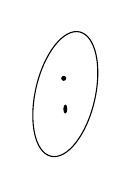
\begin{tikzpicture}[x=1cm,y=1cm]\draw[thin,rotate=-13] (0,0) ellipse (.38 and .81);\fill (-.02,.20) circle (.032); \fill (.00,-.19) ellipse (.025 and .057);\end{tikzpicture}}

% L20, between examples
Ici, $X$ \unsure{pourrait|pouvant} être variété algébrique.

% L21–23, second example
\uline{Ex 2} \unsure{\={M}} exemple \inserted{essentiellement} que le précédent, mais $Y$ étant irréductible, par exemple une droite dans le plan (\unsure{topologie|topologies} de Zariski).

% Left of L22–23, secant
\figure{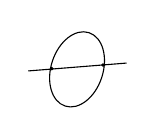
\begin{tikzpicture}[x=1cm,y=1cm]\draw[rotate=-18] (0,0) ellipse (.33 and .49);\draw (-.62,-.02)--(.63,.08);\fill (-.32,.01) circle (.025);\fill (.33,.055) circle (.025);\end{tikzpicture}}
